\documentclass[../../main.tex]{subfiles}

\begin{document}

\section{Markov Chains}

A \textbf{Markov Chain} is a stochastic process $\{X_n\}_{n=0}^\infty$ defined on a discrete state space $S$ such that the probability of transitioning to the next state depends only on the present state and not on the sequence of events that preceded it. This property is known as the \emph{Markov property}. For simplicity's sake, we assume $S$ to be finite. Hence, the formal definition:



\begin{definition}[Markov Chain]
A \textbf{Markov Chain} is a stochastic process $\{X_n\}_{n=0}^\infty$ on a discrete finite state space $S = \{1, \dots , N\}$ satisfying the \emph{Markov property}:
\[
\mathbb{P}(X_{n+1} = x_{n+1} \mid X_n = x_n, X_{n-1} = x_{n-1}, \dots, X_0 = x_0) = \mathbb{P}(X_{n+1} = x_{n+1} \mid X_n = x_n),
\]
for all $n \geq 0$ and all $x_0, \dots, x_{n+1} \in S$.

\noindent
The transition probabilities are described by a matrix $P$ with entries
\[
P_{ij} = \mathbb{P}(X_{n+1} = i \mid X_n = j), \quad \text{where } \sum_{i \in S} P_{ij} = 1 \text{ for all } j \in S.
\]
\end{definition}


\begin{example}[Markov Transition Matrix]
\label{ex:markov_chain}
Let the state space be $S = \{1, 2, 3\}$. A possible transition matrix $P$ is:
\[
P =
\begin{bmatrix}
0 & 0.7 & 0 \\
0.5 & 0.3 & 1 \\
0.5 & 0 & 0 \\
\end{bmatrix}
\]
Note that each column sums to 1.
Hence, $P$ is a valid column-stochastic Markov matrix according to the given definition.
\end{example}


\begin{remark}
    Some sources define $\bm{P'}$ s.t. $\bm{P'}_{ij} = P(X_{n+1} = j \mid X_n = i)$. The only difference is that $\bm{P'} = \bm{P}^T$.
\end{remark}


Based on these simple definitions, we can deduce very useful properties. For example, we can calculate $P(X_{t+n} = i \mid X_t = j)$ algebraically very simple based on the following result:


\begin{lemma}[n-Step Transition Probabilities]
The probability of transitioning from state $j$ to state $i$ in $n$ steps is given by the $(i,j)$-th entry of the matrix power $P^n$:
\[
\mathbb{P}(X_{t+n} = i \mid X_t = j) = (P^n)_{ij}.
\]
\end{lemma}

\begin{proof}
We prove this by induction on \( n \).

\textbf{Base case:} When \( n = 1 \), we have
\[
\mathbb{P}(X_{t+1} = i \mid X_t = j) = P_{ij} = (P^1)_{ij}.
\]

\textbf{Inductive step:} Assume the claim holds for \( n = k \), i.e.,
\[
\mathbb{P}(X_{t+k} = i \mid X_t = j) = (P^k)_{ij}.
\]
For \( n = k+1 \), using the law of total probability and the Markov property:
\[
\mathbb{P}(X_{t+k+1} = i \mid X_t = j) = \sum_{m \in S} \mathbb{P}(X_{t+k+1} = i \mid X_{t+k} = m) \cdot \mathbb{P}(X_{t+k} = m \mid X_t = j).
\]
\[
= \sum_{m \in S} P_{im} \cdot (P^k)_{mj} = (P \cdot P^k)_{ij} = (P^{k+1})_{ij}.
\]
Hence, by induction, the result holds for all \( n \geq 1 \).
\end{proof}

\begin{lemma}[n-Step Probability Distribution]
    If we have a probability distribution vector $\bm{p}_t$ at time $t$, meaning $(\bm{p}_t)_i = P(X_t = i)$, we get $\bm{p}_{t+n}$ by $\bm{P}^n \bm{p}_t$.
\end{lemma}
\vspace{-2.5em}
\begin{proof}
    \begin{align*}
        (\bm{p}_{t+n})_i &= P(X_{t+n} = i) \\
        &= \sum_{j \in S} P(X_{t+n} = i \mid X_t = j) P(X_t = j) \\
        &= \sum_{j \in S} (\bm{P}^n)_{ij} P(X_t = j) \\
        &= (\bm{P}^n \bm{p}_t)_i
    \end{align*}
\end{proof}


\subsection{Properties}
At first glance, this model seems to be very simple. However, we can characterize Markov chains by their individual properties. But what could these properties be? Well, we first might want to visualize Markov chains. To this end, we employ a graph $G = (V, E)$ with $V = S$ and $E = \{(u, v) \mid \bm{P}_{vu} \neq 0\}$.

Hence, the Markov chain from example~\ref{ex:markov_chain} becomes:

\begin{figure}[h]
    \center
    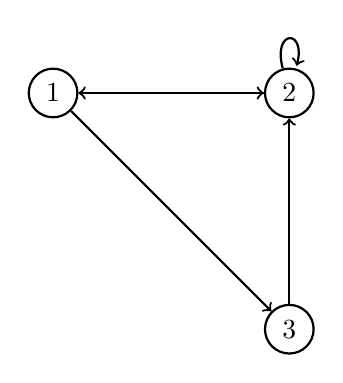
\begin{tikzpicture}[->, auto, node distance=3cm, thick]
    % Define states
    \node[circle, draw] (A) {1};
    \node[circle, draw, right of=A] (B) {2};
    \node[circle, draw, below of=B] (C) {3};

    % Transitions between states
    \draw (A) edge (B);
    \draw (A) edge (C);
    \draw (B) edge (A);
    \draw (C) edge (B);

    % Self-loops
    % \draw (A) edge[loop above] (A);
    \draw (B) edge[loop above] (B);
    % \draw (C) edge[loop below] (C);

    \end{tikzpicture}
    \caption{Graph representation of the Markov chain defined in example~\ref{ex:markov_chain}.}
    \label{fig:markov_chain}
\end{figure}

Note that we do not care about the magnitude of the transition probabilities, it only matters whether it is possible to transition from one state to another.

\subsubsection{Irreducibility}
Already we can see that we can reach every every state $v$ from every other state $u$, i.e. there exists a path of length $n$ starting at $u$ and ending at $v \iff (\bm{P}^n)_{vu} > 0$. Such a Markov chain is called \emph{irreducible}. The importance of this is that the Markov chain cannot trap itself in a subclass of states, like for example in figure~\ref{fig:markov_chain_reducible}.

\begin{figure}[h]
    \center
    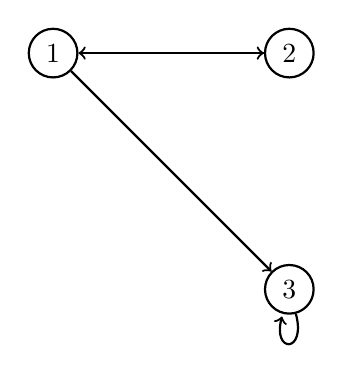
\begin{tikzpicture}[->, auto, node distance=3cm, thick]
    % Define states
    \node[circle, draw] (A) {1};
    \node[circle, draw, right of=A] (B) {2};
    \node[circle, draw, below of=B] (C) {3};

    % Transitions between states
    \draw (A) edge (B);
    \draw (B) edge (A);
    \draw (A) edge (C);

    % Self-loops
    % \draw (A) edge[loop above] (A);
    % \draw (B) edge[loop above] (B);
    \draw (C) edge[loop below] (C);

    \end{tikzpicture}
    \caption{Graph of a reducible Markov chain. Note that once the chain transitions from state $1$ to state $3$, it will stay at state $3$ indefinitely.}
    \label{fig:markov_chain_reducible}
\end{figure}

Before defining this property formally, we may first introduce a very related concept of \emph{communication classes}:

\begin{definition}
    We say that $i \in S$ \emph{leads to} state $j \in S$ iff there exists $n \in \mathbb{N}_{>0}$ s.t. $(\bm{P}^n)_{ji} > 0$. We use the notation $i \leadsto j$. Also, for all $i \in S$: $i \leadsto i$. 
\end{definition}

\begin{definition}[Communication between States]
    States $i,j \in S$ \emph{communicate} iff $i \leadsto j$ and $j \leadsto i$. We use the notation $i \leftrightsquigarrow j$.
\end{definition}

\begin{theorem}
    $i \leftrightsquigarrow j$ is an equivalence relation.
\end{theorem}
\vspace{-2.5em}
\begin{proof}
    Both reflexivity and symmetry follow directly from the definitions. For transitivity we have assuming $i \neq j$ and $j \neq k$ (the other cases are trivial):
    \begin{align*}
        &i \leftrightsquigarrow j \text{ and } j \leftrightsquigarrow k \\
        &\implies i \leadsto j \text{ and } j \leadsto i \\
        &\implies \exists_{m,n \in \mathbb{N}_{>0}} (\bm{P}^m)_{ji} > 0 \text{ and } (\bm{P}^n)_{kj} > 0 \\
        &\implies \exists_{m,n \in \mathbb{N}_{>0}} P(X_m = j \mid X_0 = i) > 0 \text{ and } P(X_{m+n} = k \mid X_m = j) > 0 \\
        &\implies P(X_{m+n} = k \mid X_0 = i) > 0 \\
        &\implies (\bm{P}^{m+n})_{ki} > 0 \\
        &\implies i \leftrightsquigarrow k
    \end{align*}
\end{proof}

Based on this result, the following definition suggests itself:

\begin{definition}[Communication Class]
    The \emph{communication class} of state $i \in S$ is the set $\{ j \in S : i \leftrightsquigarrow j \}$. This set consists of all states $j$ that communicate with $i$.
\end{definition}

\begin{remark}
    Since communication of states is an equivalence relation, the state space $S$ can be decomposed into a disjoint union of communication classes (also called a \emph{partition}). Any two communication classes either coincide completely or are disjoint sets.
\end{remark}

\begin{example}
    The partition of figure~\ref{fig:markov_chain} is $\{ \{ 1, 2, 3 \} \}$ and of figure~\ref{fig:markov_chain_reducible} we have $\{ \{ 1, 2 \} , \{ 3 \} \}$.
\end{example}

Finally, we can state the concept of \emph{irreducibility} formally:

\begin{definition}[Irreducibility]
    A Markov chain is \emph{irreducible} iff every two states communicate. Hence, an irreducible Markov chain consists of exactly one communication class.
\end{definition}

We will mostly focus on irreducible Markov chains, but for the completeness' sake we also define the following concepts:

\begin{definition}[Open and Closed Communication Class]
    A communication class $C$ is \emph{open} iff there exists a state $i \in C$ and a state $k \not \in C$ s.t. $i \leadsto k$. Otherwise, $C$ is called \emph{closed}.
\end{definition}

\begin{remark}
    An irreducible Markov chain has exactly one closed communication class.
\end{remark}

If a Markov chain once arrived in a closed communication class, it will stay in this class forever. This is exactly what happens in figure~\ref{fig:markov_chain_reducible}.

\begin{theorem}[Existence of Closed Communication Class]
    There is always at least one closed communication class.
\end{theorem}
\vspace{-2.5em}
\begin{proof}
Assume all communication classes $C_1, \dots, C_k$ are open. Hence, we can traverse these classes. But at some point we must complete a cycle, but that is a contradiction, as this would imply that those communication classes forming the cycle are really just one big communication class, which is not the case.
\end{proof}


\subsubsection{Aperiodicity}
We will now analyze the second important property of Markov chains. The reader might ask, \emph{important for what?} Well, the answer will make more sense in the big picture later, but the short answer is that these two properties will guarantee for a convergence to a unique stationary probability distribution.

To motivate the following discussion, say we had the following Markov chain:

\begin{figure}[h]
    \center
    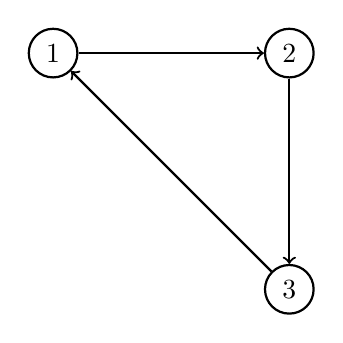
\begin{tikzpicture}[->, auto, node distance=3cm, thick]
    % Define states
    \node[circle, draw] (A) {1};
    \node[circle, draw, right of=A] (B) {2};
    \node[circle, draw, below of=B] (C) {3};

    % Transitions between states
    \draw (A) edge (B);
    \draw (B) edge (C);
    \draw (C) edge (A);

    % Self-loops
    % \draw (A) edge[loop above] (A);
    % \draw (B) edge[loop above] (B);
    % \draw (C) edge[loop below] (C);

    \end{tikzpicture}
    \caption{Graph of a periodic Markov chain. Note that once once the starting position is determined, then we also know the state after $t$ steps.}
    \label{fig:markov_chain_periodic}
\end{figure}

We notice that the behavior of this chain is periodic with a period of length $3$. Of course, this is very informal speaking, but we will now define this idea precisely.

\begin{definition}[Period and Aperiodicity]
    The \emph{period} of state $i \in S$ is defined as
    \[ \gcd \{ n \in \mathbb{N}_{>0} : (\bm{P}^n)_{ii} > 0 \} \quad . \]
    Here, $\gcd$ stands for the greatest common divisor. A state $i \in S$ is called aperiodic iff its period is equal to $1$. Otherwise, the state $i$ is called periodic.
\end{definition}

\begin{remark}
    This definition is not well defined in all cases, as it could happen that $\{ n \in \mathbb{N}_{>0} : (\bm{P}^n)_{ii} > 0 \} = \emptyset$. However, we mostly care about Markov chains being aperiodic in closed communication classes, especially in irreducible Markov chains. And for closed communication classes, this set can never be empty. In fact, for the set to be empty, we must have a communication class consisting of only one state $i \in S$ with $\bm{P}_{ii} = 0$. This communication class is obviously open.
\end{remark}

\begin{lemma}[Periodicity and Aperiodicity are Class Properties]
    If state $i \in S$ is aperiodic and $i \leftrightsquigarrow j$, then $j$ is also aperiodic.
\end{lemma}
\vspace{-2.5em}
\begin{proof}
    Since $i$ is aperiodic, we can find an $n \in \mathbb{N}$ s.t. both $(\bm{P}^n)_{ii} > 0$ and $(\bm{P}^{n+1})_{ii} > 0$ due to results from number theory. Since $j \leadsto i$, we can go from $j$ to $i$ in $t_{ji}$ steps, and from $i$ to $j$ in $t_{ij}$ steps since $i \leadsto j$. Thus:
    \[
        \{ t_{ji} + n + t_{ij}, t_{ji} + n + 1 + t_{ij} \} \subseteq \gcd \{ n \in \mathbb{N}_{>0} : (\bm{P}^n)_{jj} > 0 \} \quad .
    \]
    Since $\gcd \{ t_{ji} + n + t_{ij}, t_{ji} + n + 1 + t_{ij} \} = 1$, we conclude that $\gcd \{ n \in \mathbb{N}_{>0} : (\bm{P}^n)_{jj} > 0 \} = 1$, and hence $j$ is aperiodic.
\end{proof}

This result leads to the following definitions:

\begin{definition}[Aperiodic Markov Chain]
    An irreducible Markov chain is called aperiodic iff some (and hence, all) states in this chain are aperiodic.   
\end{definition}

With these basics covered, we can now focus on establishing important results we will need later.

\subsection{Irreducible Aperiodic Markov Chains}
We are interested in $stationary$ probability distributions $\bm{\mu}$ satisfying $\bm{P \mu} = \bm{\mu}$.

Does such a stationary probability distribution always exist? Well, for a finite state space maybe. More interestingly, we may also ask whether a Markov chain will converge towards $\bm{\mu}$ regardless of the initial probability distribution vector, i.e. for all $\bm{p}: \lim_{n \to \infty} \bm{P}^n \bm{p} = \bm{\mu} $.

In general, the answer to this is no. Consider the Markov chain in figure~\ref{fig:markov_chain_periodic} again. Clearly, if we start at certain state, say state $1$, then we will always hop around the states and never converge to $\bm{\mu}$. So our intuition might be that we need the Markov chain to be aperiodic in order for it to converge.

Furthermore, we also might ask whether the stationary probability distribution is unique. Well, in general the answer is no as well. To see this, consider this Markov chain:

\begin{figure}[h]
    \center
    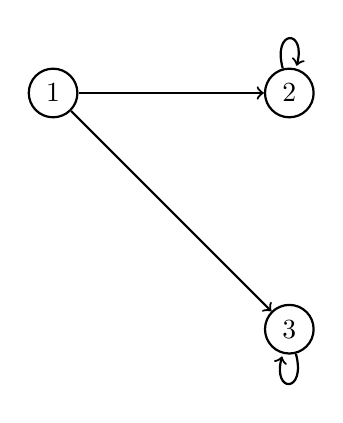
\begin{tikzpicture}[->, auto, node distance=3cm, thick]
    % Define states
    \node[circle, draw] (A) {1};
    \node[circle, draw, right of=A] (B) {2};
    \node[circle, draw, below of=B] (C) {3};

    % Transitions between states
    \draw (A) edge (B);
    \draw (A) edge (C);
    % \draw (C) edge (A);

    % Self-loops
    % \draw (A) edge[loop above] (A);
    \draw (B) edge[loop above] (B);
    \draw (C) edge[loop below] (C);

    \end{tikzpicture}
    \caption{Graph of a reducible Markov chain with two closed communication classes. Note that we might end up stuck at either state $2$ or state $3$.}
    \label{fig:markov_chain_periodic}
\end{figure}

Clearly, we have two stationary probability distributions with all their weight in either state $2$ or state $3$. Once again, our intuition tells us we might require an irreducible Markov chain.

Now it's time to specify our intuitions precisely. The following result is for irreducible aperiodic Markov chains is very significant.

\begin{theorem}[Positive n-Step Transition Matrix for Irreducible Aperiodic Markov Chains]
    For every irreducible aperiodic Markov chain specified by $\bm{P}$, there exists an $n \in \mathbb{N}_{>0}$ s.t. $\bm{P}^n > \bm{0}$, where the comparison is element-wise.
    \label{theorem:positive_transition_matrix}
\end{theorem}

We first prove the following auxiliary lemma:

\begin{lemma}
    Let $i \in S$ be an aperiodic state. Then there exists an $L \in \mathbb{N}$ s.t. for all $n > L: (\bm{P}^n)_{ii} > 0$.
    \label{lemma:aux}
\end{lemma}
\begin{proof}
    Since state $i$ is aperiodic, we can find $n_1, \dots, n_r \in \mathbb{N}$ s.t. $(\bm{P}^{n_1})_{ii} > 0, \dots, (\bm{P}^{n_r})_{ii} > 0$ and $\gcd \{ n_1, \dots , n_r \} = 1$. From number theory, we know that for $L \coloneqq \prod_{k=1}^{r} n_k$ we can write every natural number $n > L$ in the form $n = l_1 n_1 + \dots + l_r n_r$ for suitable $l_1, \dots, l_r \in \mathbb{N}$. Hence:
    \[
        (\bm{P}^{l_1 n_1 + \dots + l_r n_r})_{ii} \geq ((\bm{P}^{n_1})^{l_1})_{ii} \cdot \dots \cdot ((\bm{P}^{n_r})^{l_r})_{ii} > 0 \quad .
    \]
\end{proof}

\begin{remark}
    The converse of lemma~\ref{lemma:aux} is also true for obvious reasons.
\end{remark}

\begin{proof}[Proof of Theorem~\ref{theorem:positive_transition_matrix}]
    Let $L'$ be defined as the maximum of all $L$ defined like in Lemma~\ref{lemma:aux} when looping over all $i \in S$. Then for every $n > L'$, we have that $\bm{P}^n$ has positive entries along its diagonal. It follows that if $(\bm{P}^{t_{ji}})_{ij} > 0$ for some $t_{ji} \in \mathbb{N}_{>0}$, then we have $(\bm{P}^{n + t_{ji} + \tau})_{ij} > 0$ as well for every $\tau \in \mathbb{N}$. Furthermore, for every $i,j \in S$ we have $(\bm{P}^{t_{ji}})_{ij} > 0$ at some point $t_{ji} \in \mathbb{N}_{>0}$ due to aperiodicity. Hence, at some point all the zeros must have vanished.
\end{proof}

\begin{corollary}
    Once $\bm{P}^n > \bm{0}$, then for all $\tau \in \mathbb{N}: \bm{P}^{n + \tau} > \bm{0}$. 
\end{corollary}

The reader might question the importance of Theorem~\ref{theorem:positive_transition_matrix}. Clearly, we can see the interplay of the two properties of the Markov chain being irreducible and aperiodic in the proofs. But how does it help us finding a stationary probability distribution? Well, to answer this, we need another fundamental result, which we will cover next.


\subsection{Perron-Frobenius Theorem}
To come straight to the point, the Perron-Frobenius Theorem reads as follows:

\begin{theorem}[Perron-Frobenius]
    Let \( \bm{A} \) be a non-negative, irreducible matrix (i.e., all entries of \( \bm{A} \) are non-negative, and there exists some \( n \) such that all entries of \( \bm{A}^n \) are positive). Then the following hold:

    \begin{enumerate}
        \item The matrix \( \bm{A} \) has a unique largest non-negative eigenvalue \( \lambda_{\max} \), and this eigenvalue is simple (it has algebraic multiplicity 1).
        \item The eigenvalue \( \lambda_{\max} \) is real and positive.
        \item There is a corresponding positive eigenvector \( \bm{v} \) (i.e., all entries of \( \bm{v} \) are positive) associated with \( \lambda_{\max} \).
        \item Any other eigenvalue \( \lambda \) of \( \bm{A} \) satisfies \( |\lambda| < \lambda_{\max} \).
    \end{enumerate}
\end{theorem}

This is a mouthful, and we will not prove this theorem in this general form, as it is not trivial to do so. Instead, we focus on the case of $\bm{A}$ being a Markov chain transition matrix, meaning all columns sum to $1$. To this end, we will write $\bm{P}$ again instead of $\bm{A}$. Additionally, we assume $\bm{P}$ to be strictly positive for now instead of irreducible. Furthermore, we will not provide a rigorous proof, but we will lay the foundation for a solid intuitive understanding.

\begin{proof}[Proof of Perron-Frobenius for Positive Markov Chain Transition Matrices]
    ~\\
    Consider the mapping $T: \Delta \to \Delta$ from the unit simplex $\Delta$ onto itself defined by $T(v) \coloneqq \bm{P} v$. We want to show that $T$ is a contraction mapping with respect to the $L_1$ norm. We do this step last in order to understand the line of argument better.
    
    Thus, assume that $T$ is a contraction mapping with respect to the $L_1$ norm. By the \textsc{Banach Fixed-Point Theorem} we know that this mapping has a \emph{unique} fixed point $v^*$. We see that $v^*$ is an eigenvector of $\bm{P}$ with eigenvalue $\lambda = 1$. Clearly, $v^*$ is the only eigenvector with non-negative (actually positive!) entries, as if there were another one say $v'$, then $\frac{v'}{\|v'\|_1}$ must be one as well, but this point lies on $\Delta$, hence it must have an eigenvalue of $1$ and must be a fixed point of $T$, a contradiction to the uniqueness of $v^*$.

    So every other eigenvector $w$ with eigenvalue $\mu$ must have a coordinate-entry which is negative or truly complex. Write $|w|$ for the vector with coordinates $|w_j|$. The computation
    \[
        |\mu||w|_i = |\mu w_i| = |\sum_{j} \bm{P}_{ij} w_j| \leq \sum_{j} |\bm{P}_{ij}| |w_j| = \sum_{j} \bm{P}_{ij} |w_j| = (\bm{P} |w|)_i
    \]
    shows that $|\mu| \|w\|_1 \leq \|\bm{P} |w|\|_1 = \|w\|_1$ and hence $|\mu| \leq 1$. Now, the final trick is that we can assume the "$\leq$" in the equation above to actually be "$<$".

    To see this, note that we only have equality iff all entries of $w$ are on a line in the Gauss plane, i.e. we can write $w = c |w|$ for some $c \in \mathbb{C}, |c| = 1$. This would mean that $\bm{P} w = \bm{P} c |w| = c \bm{P} |w| \overset{!}{=} \mu w$. Hence, $\bm{P} |w| = \frac{\mu}{c} w = |\frac{\mu}{c}| |w|$. Thus, we must have $|w| = v^*$ and $|\mu| = |c| = 1$ as already discussed. Hence, $w = c v^*$ (and $\mu = 1$), which is just a different representation of the eigenvector $v^*$ already found. So for every eigenvector $w$ other than $v^*$ with eigenvalue $\mu$ we must have that $|\mu| < 1$.
\end{proof}
\end{document}